\documentclass[%
 reprint,
 amsmath,amssymb,
 aps,
 prl,
 nofootinbib,nobibnotes,
]{revtex4-2}

% \bibliographystyle{apsrev4-1}

% \usepackage{widetext}
\usepackage{graphicx}
\usepackage{tabularx}
\usepackage{dcolumn}
\usepackage{bm}
\usepackage{bold-extra}
\usepackage[ruled,vlined]{algorithm2e}

\usepackage[dvipsnames]{xcolor}
\usepackage[hidelinks]{hyperref}
\usepackage{acronym}
\usepackage{physics}
\usepackage{orcidlink}
\usepackage{xspace}
\usepackage{datatool}

\graphicspath{{plots}{plots/posterior_samples}{plots/prior_samples}}


\newacro{PE}[PE]{parameter estimation}
\newacro{GW}[GW]{gravitational-wave}
\newacro{GWTC-5}[GWTC-5]{fifth gravitational-wave transient catalog}
\newacro{GWTC-4}[GWTC-4]{fourth gravitational-wave transient catalog}
\newacro{GWTC-3}[GWTC-3]{third gravitational-wave transient catalog}
\newacro{GWTC-2}[GWTC-2]{second gravitational-wave transient catalog}
\newacro{GWTC}[GWTC]{gravitational wave transient catalog}
\newacro{LVK}[LVK]{LIGO---Virgo---KAGRA collaborations}
\newacro{O4}[O4]{fourth observing run}
\newacro{O3}[O3]{third observing run}
\newacro{HMC}[HMC]{Hamiltonian Monte Carlo}
\newacro{MC}[MC]{Monte Carlo}
\newacro{NUTS}[NUTS]{No-U-Turn Sampler}
\newacro{IID}[IID]{identically and independently distributed}
\newacro{SFR}[SFR]{star formation rate}
\newacro{KDE}[KDE]{kernel density estimate}
\newacro{BBH}[BBH]{binary black-hole}
\newacro{BNS}[BNS]{binary neutron star}
\newacro{NSBH}[NSBH]{neutron star-black hole binary}
\newacro{NS}[NS]{neutron star}
\newacro{BH}[BH]{black hole}
\newacro{GR}[GR]{general relativity}


\newacro{PISN}[PISN]{pair-instability supernova}
\newacro{PPISN}[PPISN]{pulsational pair-instability supernova}    



\newacro{PPC}[PPC]{posterior predictive check}
\newacro{MI}[MI]{mutual information}
\newacro{CAR}[CAR]{conditional autoregressive}
\newacro{ICAR}[ICAR]{intrinsic conditional autoregressive}
\newacro{PDF}[PDF]{probability density function}
\newacro{KL}[KL]{Kullback--Leibler}
\newacro{JS}[JS]{Jensen--Shannon}

\newacro{XLA}[XLA]{Accelerated Linear Algebra}
\newacro{HLV}[HLV]{Hanford, Livingston and Virgo}
\newacro{FAR}[FAR]{false-alarm rate}
\newacro{SNR}[SNR]{signal-to-noise ratio}
\newacro{IID}[IID]{independent and identically distributed}
\newacro{PSD}[PSD]{power spectral density}
\newacro{DAG}[DAG]{directed acyclic graph}


% 
% Channels
%
\newacro{CE}[CE]{common-envelope}
\newacro{OC}[OC]{open cluster}
\newacro{NSC}[NSC]{nuclear star cluster}
\newacro{CHE}[CHE]{chemically-homogeneous evolution}
\newacro{GC}[GC]{globular cluster}
\newacro{AGN}[AGN]{active galactic nuclei}
\newacro{SMT}[SMT]{stable mass transfer}

\newacro{MS}[MS]{main sequence}
\newacro{SN}[SN]{supernova}
\newacroplural{SN}[SNe]{supernovae}
\newacro{XRB}[XRB]{X-ray binary}
\newacroplural{XRB}[XRBs]{X-ray binaries}



\newacro{CAR}[CAR]{conditional auto-regressive}
\newacro{SPDE}[SPDE]{stochastic partial differential equation}
\newacro{GMRF}[GMRF]{Gaussian Markov random field}


% numbers: copies of ../macros/*.tex (notebooks/draft_figures.sh macros); use in math mode, e.g. $\peakTenMuFlex\,\Msun$.
% Found from draft/ or from the repository root.
\newcommand{\inputmacros}[1]{\IfFileExists{macros/#1.tex}{\input{macros/#1}}{\input{draft/macros/#1}}}
\inputmacros{peak_fits}
\inputmacros{joint_fits}
\inputmacros{peak_pairs}
\inputmacros{peak_excess}
\inputmacros{q_contrast}
\inputmacros{peak_odds}
\inputmacros{chi_q_broadening}
\inputmacros{peak_spins}

% math macros
\newcommand{\Msun}{\ensuremath{\mathrm{M}_{\odot}}}
\newcommand{\chieff}{\ensuremath{\chi_{\mathrm{eff}}}}
\newcommand{\chip}{\ensuremath{\chi_{\mathrm{p}}}}
\newcommand{\twoGoneG}{\ac{2G1G}\xspace}
\newcommand{\mchirp}{\ensuremath{\mathcal{M}_c}}
\newcommand{\peryear}{\ensuremath{\,\mathrm{yr}^{-1}}}

\newcommand{\red}[1]{{\color{Red} #1}}
\newcommand{\todo}[1]{{\color{Blue}\bf TODO: #1}}
\newcommand{\jh}[1]{{\color{orange}JH: #1}}
\newcommand{\comment}[1]{}
\newcommand{\PixelPop}{\textsc{PixelPop}\xspace}
\newcommand{\gwpopulation}{\textsc{GWPopulation}\xspace}
\newcommand{\BrokenPowerlawTwoPeaks}{\textsc{Broken Powerlaw Plus Two Peaks}\xspace}
\newcommand{\flexiblespins}{\textsc{Flexible}\xspace}
\newcommand{\gaussianspins}{\textsc{Gaussian}\xspace}
% feature labels: approximate measured locations (m1 in Msun); macro names keep the old round numbers
\newcommand{\featTen}{10\xspace}
\newcommand{\featTwenty}{21\xspace}
\newcommand{\featThirtyFive}{33\xspace}
\newcommand{\featSixty}{59\xspace}


\newcommand{\heading}[1]{\textbf{\textit{#1}}}

\begin{document}

\title{Nonparametric mass and spin inference reveals peaks and correlations \jh{title sucks, tbd}}

\author{Jack Heinzel\,\orcidlink{0000-0002-5794-821X}}
\email{jheinzel@flatironinstitute.org}

\author{Matthew Mould\,\orcidlink{}}


\date{\today}

\begin{abstract}
abstracto petronum

% \red{Abstract ($\le 600$ characters), one sentence each: the data (259 events, GWTC-5 / O4b); the method (nonparametric, no templates); the result (near-equal-mass peaks at $\jointTenMuFlex\,\Msun$ and $\jointThirtyFiveMuFlex\,\Msun$; $q\approx 0.5$ peaks at $\jointTwentyMuFlex\,\Msun$ and $\jointSixtyMuFlex\,\Msun$, about twice the mass, with broad $\chieff$ there); the meaning (consistent with hierarchical mergers; tentative; the full O4 sample will decide).}
\end{abstract}

\maketitle

\heading{Introduction.}
With more than 250 \ac{BBH} mergers now cataloged by the LIGO~\cite{LIGOScientific:2014pky}, Virgo~\cite{VIRGO:2014yos}, and KAGRA~\cite{KAGRA:2020tym} detectors~\cite{LIGOScientific:2018mvr, LIGOScientific:2020ibl, LIGOScientific:2021usb, KAGRA:2021vkt, LIGOScientific:2025slb, LIGOScientific:2026wfs}, we are beginning to reveal the structure of the \ac{BBH} population. The \ac{BH} mass distribution has a prominent peak at $\sim 10\Msun$~\cite{LIGOScientific:2020kqk, Tiwari:2020otp, Edelman:2021zkw, KAGRA:2021duu, Callister:2023tgi, LIGOScientific:2025pvj, LIGOScientific:2026ctl}, a feature at $\sim 30$--$35 \Msun$ which may be a local peak or steepening~\cite{Talbot:2018cva, LIGOScientific:2020kqk, KAGRA:2021duu, Farah:2023vsc, LIGOScientific:2025pvj, LIGOScientific:2026ctl}, and a tail that extends into the theorized \ac{PISN} mass gap~\cite{Barkat:1967zz, Woosley:2016hmi, Tong:2025wpz, Antonini:2025ilj, Ray:2025xti}. Most \ac{BH} spins are small~\cite{Miller:2020zox, Roulet:2021hcu, Callister:2022qwb, Tong:2022iws, KAGRA:2021duu}, though there exists a subpopulation of rapid spins~\cite{Antonini:2024het, Plunkett:2026pxt, Li:2025iux, LIGOScientific:2026ctl}, and the astrophysical \ac{BBH} merger rate increases with redshift~\cite{Fishbach:2018edt, LIGOScientific:2020kqk, KAGRA:2021duu, LIGOScientific:2026ctl}. 
The population of \ac{BBH} is \textit{correlated} as well. The effective spin~\cite{Damour:2001, Racine:2008qv, Ajith:2009bn} distribution appears to broaden with mass ratio~\cite{Callister:2021fpo, Adamcewicz:2022hce, Heinzel:2023hlb, LIGOScientific:2026ctl}, redshift~\cite{Biscoveanu:2022qac, Heinzel:2023hlb}, and appears to have a nontrivial narrow-broad-narrow-broad structure across the mass distribution~\cite{Antonini:2025ilj, Tong:2025xir, Plunkett:2026pxt, Flanagan:2026ayy, Alvarez-Lopez:2026ymo} \jh{fix that sentence}. 

\jh{maybe something about astrophysics...?}
Most of population results come from models that assume the population is uncorrelated or let a single pair of binary parameters correlate while holding the rest to a fixed, usually parametric, form. The $q$--$\chieff$ correlation, for example, is typically measured with a mass distribution that does not depend on spin, and the mass spectrum with a single mass ratio distribution at every primary mass. Each conclusion is therefore conditional on assumptions that other analyses relax. A fully joint model is computationally demanding, and for the smaller catalogs of a few dozen events, correlations among all the parameters at once were too subtle to detect \citep[e.g., ][]{Biscoveanu:2022qac}. With hundreds of \acp{BBH}, this is no longer true.

Here we fit the masses, mass ratio and spins jointly, letting each distribution correlate in an unspecified, flexible manner. Towards equal mass ratios, the primary mass spectrum peaks at $m_1 = \jointTenMuFlex\,\Msun$ and $\jointThirtyFiveMuFlex\,\Msun$ (mean $q = \jointTenQMeanFlex$ and $\jointThirtyFiveQMeanFlex$, but consistent with \textit{peaking} at $q\to 1$). The mean mass ratio falls away from these peaks, and at $q \sim 0.5$ we find \jh{todo: macros} $\textcolor{red}{XX.X\%}$ evidence for a second pair of peaks, at $m_1 = \jointTwentyMuFlex\,\Msun$ and $\jointSixtyMuFlex\,\Msun$ (mean $q = \jointTwentyQMeanFlex$ and $\jointSixtyQMeanFlex$), about twice the masses of the first. The spin behavior also splits aligned with the mass ratios: the near-equal-mass peaks have a narrow effective spin distribution, while the $q \sim 0.5$ peaks have a broad, nearly symmetric one, as expected from large, isotropically oriented spins.

We also show that the separation into two families of peaks with different mass ratios and spin properties explains the broadening $\chieff$ with mass ratio, a correlation identified in \citet{LIGOScientific:2026ctl}, and are consistent with the spin correlations identified in Refs.~\cite{Antonini:2025ilj, Tong:2025xir, Plunkett:2026pxt, Flanagan:2026ayy}. These mass peaks appear remarkably consistent with a dynamical \twoGoneG, where a first generation \ac{BH} merges with the remnant of a previous \ac{BBH} merger. We show the observed primary mass in the $q\sim 0.5$ features are consistent with the expected remnant masses from mergers in the $q\sim 1$ features (assuming \ac{GR}) \jh{some tension in 20M peak}. 

\heading{Methods.}
We infer the population of \acp{BBH} following \ac{GWTC-5},  using the same dataset of 259 \acp{BBH} with \ac{FAR} $<1\peryear$ and sensitivity estimates as described in \citet{LIGOScientific:2026ctl}. We use the hierarchical Bayesian inference framework, with details described in the supplemental material.

We consider a pair of flexible models which model the joint distribution of primary mass $m_1$, mass ratio $q$, and effective aligned and precessing spins $\chieff$ and $\chip$, respectively. We decompose the distribution as
\begin{equation}
    p(m_1, q, \chieff, \chip, z) = p(m_1, q)p(\chieff, \chip \mid m_1, q)p(z),
    \label{eq: spins conditional on mass basic model}
\end{equation}
where the redshift distribution is assumed to be uncorrelated and evolves according to the \textsc{Power Law Redshift} model introduced in Ref.~\citet{Fishbach:2018edt}.

We model the joint distribution of $p(m_1, q)$ as a two-dimensional Mat\'ern field using \PixelPop. We model the conditional $p(\chieff, \chip \mid m_1, q)$ using a pair of models. The \flexiblespins model treats $p(\chieff, \chip \mid m_1, q)$ as a separate, four dimensional \PixelPop Mat\'ern field normalized along each $m_1, q$ (details in the supplemental material). Our \gaussianspins model treats
\begin{equation}
    p(\chieff, \chip \mid m_1, q) = \mathcal{N}\big(\vec{\mu}, C\big)
\end{equation}
as a bivariate Gaussian distribution, whose mean $\mu_{\chieff}, \mu_{\chip}$, standard deviation $\sigma_{\chieff}, \sigma_{\chip}$ and correlation coefficient $\rho$ are each two-dimensional \PixelPop Mat\'ern fields over $(m_1, q)$, truncated to the effective spins physical domain (Eq.~12 of \citet{iwaya_analytic_2025}). We also consider variations where the mean and standard deviation evolve separately, described in the supplemental material.  

Though a Gaussian model may be misspecified against the astrophysical shape of the $\chieff, \chip$ population, Gaussian models are attractive for their interpretative abilities: we may directly interpret the measured moments against their prior. The \flexiblespins model allows for generic, non-Gaussian spin distributions that evolve with mass, but it induces a nontrivial prior on the implied moments (mean and standard deviation) of the spin distribution. For instance, the \flexiblespins model preferentially \textit{broadens} in regions which are poorly constrained by the data, as the model reverts to the smooth field prior. Data-poor regions in the \gaussianspins model, by contrast, should correspond to broader \textit{uncertainties} on the moments, as opposed to biases. \jh{check in final runs:} In practice, we observe similar constraints on the population moments for both models.

\heading{Mass features.}
We show the inferred binary mass distribution in Fig.~\ref{fig: mass peaks}. In the top panel, we compare the marginal primary mass distribution with slices of primary mass with mass ratio close to 1, and with mass ratio close to $q\sim 1/2$. For mass ratios $q\in [0.8,1]$, the primary mass spectrum has a pair of peaks at $\sim$ \featTen $\Msun$ and $\sim$ \featThirtyFive $\Msun$; for mass ratios $q\in [0.3,0.65]$, the mass spectrum shows \textit{different} peaks at $\sim$ \featTwenty $\Msun$ and $\sim$ \featSixty $\Msun$.

\begin{figure}
    \centering
    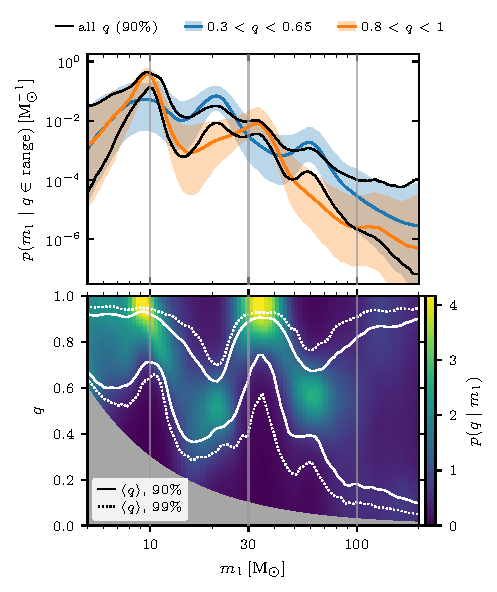
\includegraphics[width=\linewidth]{draft/plots/mass_ratio_m1.pdf}
    \caption{\textit{Top}: the primary-mass distribution $p(m_1)$  integrated over all mass ratios (black lines for 90\% interval) and restricted to $0.3 < q < 0.65$ (blue) and $0.8 < q < 1$ (orange) (90\% bands and medians), for the flexible spin model. 
    \textit{Bottom}: the median $p(q \mid m_1)$, with the 90\% (solid) and 99\% (dashed) intervals of the mean mass ratio $\langle q \rangle$ at each $m_1$. Peaks at $\sim$ \featTen $\Msun$ and $\sim$ \featThirtyFive $\Msun$ prefer near equal masses, while an additional pair of peaks at $\sim$ \featTwenty $\Msun$ and $\sim$ \featSixty $\Msun$ emerge at mass ratios $q\sim 0.5$.}
    \label{fig: mass peaks}
\end{figure}

\begin{table}
    \renewcommand{\arraystretch}{1.3}
    \caption{Properties of the four mass peaks in the \flexiblespins model (medians and 90\% intervals; \gaussianspins values in the SM). The mean and width $\mu$ and $\sigma$ come from direct fits to $p(m_1 \mid q \in [0.8,1])$ or $p(m_1 \mid q \in [0.3,0.65])$, described in SM. The mean and mode of the mass ratio, $\langle q \rangle$ and $q_{\rm mode}$, are computed directly from $p(m_1, q)$ for $m_1$ integrated over $[8, 12]$, $[15, 25]$, $[28, 40]$ and $[50, 70]\,\Msun$. The mass ratio mode $q_{\rm mode}$ is noisy for the \featTwenty and \featSixty $\Msun$ features: where $p(q \mid m_1)$ is broad, small fluctuations can shift its maximum substantially.}
    \label{tab: peaks}
    \begin{ruledtabular}
    \begin{tabular}{lcccc}
        Peak & $\mu$ [\Msun] & $\sigma$ [\Msun] & $\langle q \rangle$ & $q_{\rm mode}$ \\
        \hline
        \featTen & $\peakTenMuFlex$ & $\peakTenSigmaFlex$ & $\qWindowTenFlex$ & $\qModeWindowTenFlex$ \\
        \featTwenty & $\peakTwentyMuFlex$ & $\peakTwentySigmaFlex$ & $\qWindowTwentyFlex$ & $\qModeWindowTwentyFlex$ \\
        \featThirtyFive & $\peakThirtyFiveMuFlex$ & $\peakThirtyFiveSigmaFlex$ & $\qWindowThirtyFiveFlex$ & $\qModeWindowThirtyFiveFlex$ \\
        \featSixty & $\peakSixtyMuFlex$ & $\peakSixtySigmaFlex$ & $\qWindowSixtyFlex$ & $\qModeWindowSixtyFlex$ \\
    \end{tabular}
    \end{ruledtabular}
\end{table}


\todo{plots comparing fits to nonparametrics go into the SM}

\jh{is this too much detail}
To extract parameters for each feature, we fit a Gaussian plus a power-law continuum to the primary mass distribution in a fixed window, restricted to the mass-ratio range in which the feature appears (windows in the SM). We report the mean and width of the Gaussian, $\mu$ and $\sigma$, as the location and width of the feature (Table~\ref{tab: peaks}). \jh{say what we do with fits that land on boundaries} % We repeat the fit for each posterior draw, so the quoted intervals reflect the uncertainty in the inferred distribution; in more than $98\%$ of draws, the fit places the Gaussian inside the window rather than at its edge. This is not intended as an optimal estimator of the shape of each feature, but as a simple summary of the data-driven inference. 
To check that each feature is localized in mass ratio as well as in primary mass, we also fit a two-component model in $(m_1, q)$ within the same windows, with no mass-ratio range imposed. Both fits are described in the SM.

The global peak of the \ac{BH} mass spectrum is at $m_1 = \peakTenMuFlex\,\Msun$, with a narrow width $\sigma = \peakTenSigmaFlex\,\Msun$ (Table~\ref{tab: peaks}). This \featTen $\Msun$ feature has been prominent since catalogs were a few dozens of events~\cite[e.g.,][]{LIGOScientific:2020kqk, Talbot:2018cva, Tiwari:2020otp, Edelman:2021zkw, KAGRA:2021duu, Callister:2023tgi}, and is now firmly established~\cite{LIGOScientific:2025pvj, LIGOScientific:2026ctl}. We find that \acp{BBH} in this feature prefer equal-mass pairing ($q_{\rm mode} = \qModeWindowTenFlex$, $\langle q \rangle = \qWindowTenFlex$), consistent with~\cite{Farah:2023swu, LIGOScientific:2026ctl, Flanagan:2026ayy}, and in mild tension with some claims of a mass ratio distribution peaking away from unity at \featTen $\Msun$~\cite{Godfrey:2023oxb, Sadiq:2023zee, Sridhar:2025kvi, LIGOScientific:2025pvj}. A peak near \featThirtyFive $\Msun$ was also observed in early population analyses~\cite{Talbot:2018cva, LIGOScientific:2018jsj, LIGOScientific:2020kqk, KAGRA:2021duu, Farah:2023vsc}, with near-equal masses~\cite{Roy:2025ktr, Sridhar:2025kvi}, but the \ac{LVK} showed that the marginal primary mass distribution is consistent with either a peak \textit{or} a steepening~\cite{LIGOScientific:2025pvj, LIGOScientific:2026ctl}. For $q \in [0.8, 1]$, however, we observe stronger evidence for a peak: the merger rate rises into the $30$--$35\,\Msun$ window as well as falling after it, with posterior-to-prior odds $\mathcal{O}_{\rm peak} = \peakOddsHiBFFlex$, against $\peakOddsAllBFFlex$ over all mass ratios (see the SM). The difference comes from the low-mass side of the feature: the \featTwenty $\Msun$ feature populates the region between \featTen and \featThirtyFive $\Msun$ at unequal mass ratios, filling in the rise toward \featThirtyFive $\Msun$ in the marginal distribution. We argue the \featThirtyFive $\Msun$ feature should therefore be located by \textit{both} its mass and its mass ratio. % We argue this clarifies the degeneracy identified by \citet{LIGOScientific:2025pvj}: the steepening seen in the marginal distribution is what a near-equal-mass peak looks like once the unequal-mass binaries from the \featTwenty $\Msun$ feature are averaged in.

For $q \in [0.3, 0.65]$, the mass spectrum instead peaks at $m_1 = \peakTwentyMuFlex\,\Msun$ and $\peakSixtyMuFlex\,\Msun$, with mean mass ratios $\langle q \rangle = \qWindowTwentyFlex$ and $\qWindowSixtyFlex$, respectively. Neither feature appears in the near-equal-mass $q\in [0.8,1]$ slice of Fig.~\ref{fig: mass peaks}. Within $q \in [0.3, 0.65]$, the merger rate at each exceeds a local power law with posterior probability $\peakTwentyExcessPLocFlex\%$ and $\peakSixtyExcessPLocFlex\%$ (c.f.\ $\peakTwentyExcessPLocPriorFlex\%$ and $\peakSixtyExcessPLocPriorFlex\%$ under the prior). Earlier analyses with weakly parameterized models reported hints of additional structure near $20\,\Msun$~\cite{Tiwari:2020otp, Tiwari:2021yvr, Edelman:2022ydv, Toubiana:2023egi, MaganaHernandez:2024uty} and $60\,\Msun$~\cite{MaganaHernandez:2024uty, LIGOScientific:2025pvj}, but \citet{LIGOScientific:2026ctl} found no evidence for either in the \ac{GWTC-5} primary mass distribution. In the marginal distribution, the \featTwenty $\Msun$ feature is weak because it sits between the much larger \featTen and \featThirtyFive $\Msun$ features; it becomes clearer only once the mass ratio is specified. \citet{LIGOScientific:2026ctl} did find a flatter mass ratio distribution above $m_1 \sim 40\,\Msun$, together with a change in spin properties, consistent with hierarchical mergers. Our result is in line with this, and resolves it further: the unequal-mass binaries above $\sim 40\,\Msun$ are concentrated around \featSixty $\Msun$ rather than spread across the high-mass tail. The \featSixty $\Msun$ feature is the least well measured of the four, and we regard both unequal-mass features as tentative. We discuss each feature in detail in the SM.

We should note that we identified these features (and chose the windows in which we fit them) after inspecting the inferred distribution. This procedure is known to inflate statistical significance (the ``look-elsewhere'' effect~\cite[e.g.,][]{Gross:2010qma}). A finite catalog drawn from a featureless population occasionally produces overdensities somewhere in $(m_1, q)$, an effect we do not attempt to account for. A proper calibration would require repeating our procedure on catalogs drawn from featureless populations~\cite[e.g.,][]{Farah:2023vsc}, which we leave to future work. However, independent of their separation in mass, which we used to assess their significance, we also identify a bifurcation in the spin behavior of the two families of peaks. \jh{do we move this discussion to the end?}

%along the . First, the \featTen and \featThirtyFive $\Msun$ peaks are well-known features in the \ac{GW} population\jh{cite ...}. Second, the four features have distinct \textit{spin} properties: the $\chieff$ distribution is narrow at the \featTen and \featThirtyFive $\Msun$ peaks (centered on $\chieff > 0$ for \featTen $\Msun$ and consistent with a $\chieff =0$ mean for \featThirtyFive $\Msun$)  and broad at the \featTwenty and \featSixty $\Msun$ features (Table~\ref{tab: spins}).

\todo{check samples are they affected by RIFT EOB issue} \jh{we are good!}

\heading{Spin properties.}
The four features also differ in their spins (Fig.~\ref{fig: spin peaks} and Table~\ref{tab: spins}). The $\sim \featTen\,\Msun$ feature is the only mass at which the mean of the $\chieff$ distribution is confidently positive: $\mu_{\chieff} = \peakSpinTenEffMeanCoreFlex$ ($\peakSpinTenEffMeanCoreGauss$) in the \flexiblespins (\gaussianspins) model, positive with $\peakSpinTenPEffPosFlex\%$ ($\peakSpinTenPEffPosGauss\%$) credibility, and the distribution of $\chieff$ is narrow: $\sigma_{\chieff} = \peakSpinTenEffSdCoreFlex$ ($\peakSpinTenEffSdCoreGauss$). The precessing spins are also small, $\mu_{\chip} = \peakSpinTenPMeanFlex$ ($\peakSpinTenPMeanGauss$). Large in-plane spins are therefore ruled out: together with the narrow $\chieff$ distribution, this indicates the black holes at $\sim\featTen \,\Msun$ have small spin magnitudes, not only small \textit{aligned} components. The nonzero lower bound on $\mu_{\chip}$, however, should not be taken as evidence for misaligned spins. $\chip$ is positive by construction and poorly measured for individual events, particularly for near-equal masses~\cite{Apostolatos:1994mx, Green:2020ptm}, so populations with \textit{small} vs \textit{zero} in-plane spins are remarkably difficult to distinguish~\cite[e.g.][]{Vitale:2022dpa, Miller:2024sui, Vitale:2025lms}. 

\jh{move to a new section on interpretation...?}
Near-equal masses with small, aligned spins are the expected signature of binaries that evolved together (e.g., in the field or as an original binary in young/open star cluster) ~\cite{Zaldarriaga:2017qkw, Qin:2018vaa, Fuller:2019sxi, DiCarlo:2019pmf, Bavera:2020inc, Zevin:2022wrw}, rather than assembled dynamically. The preferentially-aligned spins indicate that the $\sim \featTen\,\Msun$ peak is therefore unlikely to be entirely dynamical; we overview the possible formation channels for the \featTen $\Msun$ peak in the SM. 
The \featThirtyFive $\Msun$ feature also has a narrow $\chieff$ distribution. Importantly, however, the mean at $m_1 \sim \featThirtyFive \,\Msun$ is consistent with zero, $\mu_{\chieff}=\peakSpinThirtyFiveEffMeanCoreFlex$ ($\peakSpinThirtyFiveEffMeanCoreGauss$ with the \gaussianspins model), which suggests that it \textit{is} possible to assemble the entire $\sim \featThirtyFive$ $\Msun$ feature dynamically. 

The unequal-mass features, in contrast, have a broad effective spin distribution consistent with symmetry about zero, and larger precessing spins are preferred (Table~\ref{tab: spins}). At the \featTwenty $\Msun$ feature, $\mu_{\chieff} = \peakSpinTwentyEffMeanCoreFlex$ and $\sigma_{\chieff} = \peakSpinTwentyEffSdCoreFlex$ ($\peakSpinTwentyEffMeanCoreGauss$ and $\peakSpinTwentyEffSdCoreGauss$ with the \gaussianspins model), and at the \featSixty $\Msun$ feature, $\mu_{\chieff} = \peakSpinSixtyEffMeanCoreFlex$ and $\sigma_{\chieff} = \peakSpinSixtyEffSdCoreFlex$ ($\peakSpinSixtyEffMeanCoreGauss$ and $\peakSpinSixtyEffSdCoreGauss$). These widths are two to three times those of the near-equal-mass features, and both are consistent with $\sigma_{\chieff} \approx 0.27$, the width expected when the primary is a previous merger remnant ($\chi\sim0.69$) with isotropic spins and a mass ratio $q\sim 1/2$ ($\sigma_{\chieff} = 0.27$ is the standard deviation of $U(-0.47, 0.47)$, the uniform \twoGoneG $\chieff$ distribution of Ref.~\cite{Antonini:2024het} \jh{are there other relevant citations}). The precessing spins are also somewhat larger at the unequal-mass features (Fig.~\ref{fig: spin peaks}), but $\chip$ is not measured far from the prior: $\mu_{\chip} = \peakSpinTwentyPMeanFlex$ and $\peakSpinSixtyPMeanFlex$, against $\peakSpinTwentyPMeanPriorFlex$ under the prior. \jh{for later: the \featTwenty $\Msun$ $\mu_{\chip}$ is below the \twoGoneG expectation but (a) $\chip$ is finicky and I suspect smoothed by the prior mostly, though (b) maybe this goes along with the mass mapping $\featTen \to \featTwenty$ not quite working.}

Together, the narrow spins of the near-equal-mass features and the broad spins of the unequal-mass features account for the broadening of the $\chieff$ distribution toward unequal masses~\cite{Callister:2021fpo, Adamcewicz:2023mov, LIGOScientific:2026ctl} and for its narrow--broad--narrow--broad structure in primary mass~\cite{Antonini:2025ilj, Tong:2025xir, Plunkett:2026pxt, Flanagan:2026ayy}, as we show in the End Matter.

\begin{figure*}
    \centering
    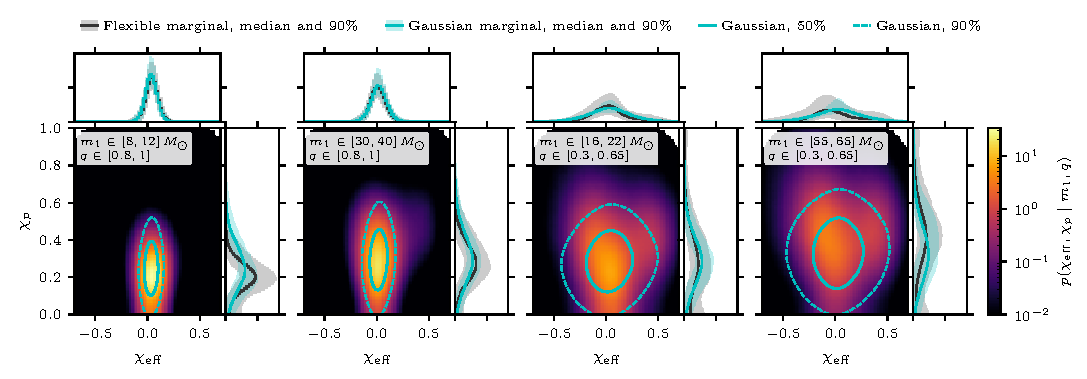
\includegraphics[width=\linewidth]{draft/plots/spin_peak_regions_marginals.pdf}
    \caption{\red{Draft caption. The joint spin distribution $p(\chieff, \chip \mid m_1, q)$ in the four peak regions: the two near-equal-mass peaks ($m_1 \in [8, 12]$ and $[30, 40]\,\Msun$, $q \in [0.8, 1]$) and the two $q \approx 0.5$ peaks ($m_1 \in [16, 22]$ and $[55, 65]\,\Msun$, $q \in [0.3, 0.65]$). Heatmap: the flexible spin model's median density (shared logarithmic colour scale); black contour: the Gaussian spin model's 90\% region. Side panels: the marginals $p(\chieff \mid m_1, q)$ (top) and $p(\chip \mid m_1, q)$ (right), for the flexible model the median and 90\% band over posterior draws (orange), for the Gaussian model the 90\% band (black lines). The near-equal-mass peaks have narrow, slightly positive $\chieff$; the $q \approx 0.5$ peaks have broad, nearly symmetric $\chieff$ and larger $\chip$. The grey corner is outside the physical $(\chieff, \chip)$ range, $\chip > \chi_{p,\max}(\chieff, q)$ at the largest $q$ of the region. \todo{Calculate positive vs negative statistic for Xeff} }}
    \label{fig: spin peaks}
\end{figure*}

\begin{table*}
    \renewcommand{\arraystretch}{1.3}
    \caption{Spin properties of the four features: the mean and standard deviation of $\chieff$ (restricted to the core, $|\chieff| < 0.8$) and of $\chip$ in each feature's region, and the probability that the mean $\chieff$ is positive (medians and 90\% intervals; \flexiblespins and \gaussianspins models). Regions: $m_1 \in [8, 12]$ and $[30, 40]\,\Msun$ for $q \in [0.8, 1]$; $m_1 \in [16, 22]$ and $[55, 65]\,\Msun$ for $q \in [0.3, 0.65]$. Last row: the expectation for a second-generation primary with spin $\chi_f = 0.69$, isotropically oriented, and a nonspinning first-generation secondary at $q = 0.5$ (SM). \todo{}}
    \label{tab: spins}
    \begin{ruledtabular}
    \small
    \setlength{\tabcolsep}{1.8pt}
    \begin{tabular}{l | ccccc | ccccc}
        & \multicolumn{5}{c|}{\flexiblespins} & \multicolumn{5}{c}{\gaussianspins} \\
        \cline{2-11}
        Feature & $\mu_{\chieff}$ & $\sigma_{\chieff}$ & $\mu_{\chip}$ & $\sigma_{\chip}$ & $P(\mu_{\chieff} > 0)$ & $\mu_{\chieff}$ & $\sigma_{\chieff}$ & $\mu_{\chip}$ & $\sigma_{\chip}$ & $P(\mu_{\chieff} > 0)$ \\
        \hline
        \featTen $\Msun$ & $\peakSpinTenEffMeanCoreFlex$ & $\peakSpinTenEffSdCoreFlex$ & $\peakSpinTenPMeanFlex$ & $\peakSpinTenPSdFlex$ & $\peakSpinTenPEffPosFlex\%$ & $\peakSpinTenEffMeanCoreGauss$ & $\peakSpinTenEffSdCoreGauss$ & $\peakSpinTenPMeanGauss$ & $\peakSpinTenPSdGauss$ & $\peakSpinTenPEffPosGauss\%$ \\
        \featThirtyFive $\Msun$ & $\peakSpinThirtyFiveEffMeanCoreFlex$ & $\peakSpinThirtyFiveEffSdCoreFlex$ & $\peakSpinThirtyFivePMeanFlex$ & $\peakSpinThirtyFivePSdFlex$ & $\peakSpinThirtyFivePEffPosFlex\%$ & $\peakSpinThirtyFiveEffMeanCoreGauss$ & $\peakSpinThirtyFiveEffSdCoreGauss$ & $\peakSpinThirtyFivePMeanGauss$ & $\peakSpinThirtyFivePSdGauss$ & $\peakSpinThirtyFivePEffPosGauss\%$ \\
        \featTwenty $\Msun$ & $\peakSpinTwentyEffMeanCoreFlex$ & $\peakSpinTwentyEffSdCoreFlex$ & $\peakSpinTwentyPMeanFlex$ & $\peakSpinTwentyPSdFlex$ & $\peakSpinTwentyPEffPosFlex\%$ & $\peakSpinTwentyEffMeanCoreGauss$ & $\peakSpinTwentyEffSdCoreGauss$ & $\peakSpinTwentyPMeanGauss$ & $\peakSpinTwentyPSdGauss$ & $\peakSpinTwentyPEffPosGauss\%$ \\
        \featSixty $\Msun$ & $\peakSpinSixtyEffMeanCoreFlex$ & $\peakSpinSixtyEffSdCoreFlex$ & $\peakSpinSixtyPMeanFlex$ & $\peakSpinSixtyPSdFlex$ & $\peakSpinSixtyPEffPosFlex\%$ & $\peakSpinSixtyEffMeanCoreGauss$ & $\peakSpinSixtyEffSdCoreGauss$ & $\peakSpinSixtyPMeanGauss$ & $\peakSpinSixtyPSdGauss$ & $\peakSpinSixtyPEffPosGauss\%$ \\
        \hline
        \twoGoneG & $0$ & $0.27$ & $0.54$ & $0.15$ & -- & $0$ & $0.27$ & $0.54$ & $0.15$ & -- \\
    \end{tabular}
    \end{ruledtabular}
\end{table*}

\heading{Hierarchical mergers.}
The location, mass ratio and spins of the unequal-mass features are what one qualitatively expects of second-generation mergers built from the near-equal-mass features. Two $\sim$\featTen $\Msun$ black holes merge into a remnant of $\sim 18\,\Msun$ with spin $\chi \approx 0.7$; if the remnant merges again with another $\sim \featTen$ $\Msun$ first-generation black hole (a \twoGoneG merger), the binary has $q \approx 0.5$, and if it is assembled dynamically, its spins are isotropically oriented, giving a broad, symmetric $\chieff$ distribution~\cite{Fishbach:2017dwv, Gerosa:2017kvu, Rodriguez:2019huv, Gerosa:2021mno, Ginat:2026awh}. Likewise, two $\sim$\featThirtyFive $\Msun$ black holes merge into a remnant of $\sim 60\,\Msun$. This lies in the pair-instability mass gap, whose lower edge has been placed near $\sim 45\,\Msun$ using the secondary masses and spins of \ac{GWTC-4} binaries~\cite{Tong:2025wpz, Antonini:2025ilj}, though see~\cite{Ray:2025xti}. Such black holes cannot form directly from stellar collapse, but can be the remnants of earlier mergers~\cite{Rodriguez:2019huv, Kimball:2020opk, Gerosa:2021mno, Antonini:2024het}, and hierarchical subpopulations at high mass have also been argued for in \ac{GWTC-4}~\cite[e.g.,][]{Plunkett:2026pxt, Li:2025iux}. We test the coherence of this picture in mass ratio, primary mass and spin.

% \textit{Mass ratio.} 
In both pairs of peaks, the mean mass ratio drops from $\langle q \rangle \approx 0.85$ at the near-equal-mass feature to $\approx 0.55$ at the unequal-mass one. The difference in means are $\Delta_{\featTen,\featTwenty} = \qContrastTenTwentyMedFlex$, $\Delta_{\featThirtyFive,\featTwenty} = \qContrastThirtyFiveTwentyMedFlex$ and $\Delta_{\featThirtyFive,\featSixty} = \qContrastThirtyFiveSixtyMedFlex$, \red{with posterior probabilities $P(\Delta > 0) = \qContrastTenTwentyPFlex\%$, $\qContrastThirtyFiveTwentyPFlex\%$ and $\qContrastThirtyFiveSixtyPFlex\%$} (SM). % The $m_2 > 3\,\Msun$ cut offsets $\Delta_{\featTen,\featTwenty}$ under the prior ($\qContrastTenTwentyMedPriorFlex$); measured against this offset, $Z_{\rm shift} = \qContrastTenTwentyZShiftFlex$.

\textit{Masses.} If the unequal-mass features are second-generation mergers, their primary mass is the remnant of the lower feature, $\approx 95\%$ of its total mass (SM). We measure the retained fraction $m_{1,\rm hi}/M_{\rm lo}$ without fitting, from the mode of $p(m_1 \mid 0.3 < q < 0.65)$ at the higher feature and the mode of the total mass $M = m_1(1 + q)$ of the lower one (Fig.~\ref{fig: bookkeeping}). For $\featThirtyFive \to \featSixty$, $m_{1,\rm hi}/M_{\rm lo} = \pairThirtyFiveSixtyRetainedModeFlex$, consistent with $\sim 5\%$ radiated. For $\featTen \to \featTwenty$, $m_{1,\rm hi}/M_{\rm lo} = \pairTenTwentyRetainedModeFlex$, with 0.95 at the $\pairTenTwentyQuantileRetainedModeFlex\%$ quantile: a mild tension, with the \featTwenty $\Msun$ feature slightly above the expected location. The dynamical first-generation spectrum may differ from the (field-dominated, $\chieff > 0$) \featTen $\Msun$ peak, or the pairing may be selective; this model cannot separate the channels (SM).

\textit{Spins.} A second-generation primary with spin $\chi_f \approx 0.69$, isotropically oriented and paired with a slowly spinning first-generation secondary, has $\chieff \approx \chi_f \cos\theta_1/(1 + q)$ and $\chip \approx \chi_f \sin\theta_1$. At $q = 0.5$ this gives $\mu_{\chieff} = 0$, $\sigma_{\chieff} = \chi_f/[(1 + q)\sqrt{3}] \approx 0.27$, $\mu_{\chip} = \pi\chi_f/4 \approx 0.54$ and $\sigma_{\chip} \approx 0.15$ (Table~\ref{tab: spins}; SM). The effective spins of the \featTwenty and \featSixty $\Msun$ features match this: their means are consistent with zero, and their widths, $\sigma_{\chieff} = \peakSpinTwentyEffSdCoreFlex$ and $\peakSpinSixtyEffSdCoreFlex$, with 0.27. Their mean precessing spins, $\mu_{\chip} = \peakSpinTwentyPMeanFlex$ and $\peakSpinSixtyPMeanFlex$, are lower than expected, most clearly at the \featTwenty $\Msun$ feature. Each region also contains first-generation binaries with smaller spins, and a second-generation fraction $f < 1$ lowers both the mean $\chip$ and the width of $\chieff$ (SM). \jh{evaluate $f$ from the peak fractions: roughly, $\mu_{\chip}$ at \featTwenty $\Msun$ gives $f \sim 0.3$, and $\sigma_{\chieff}$ gives $f \sim 0.6$.} Hierarchical mergers in active galactic nuclei disks would instead produce preferentially aligned spins, and so positive $\chieff$ at low mass ratio~\cite{Li:2025iux}; the means we find are consistent with zero, which favors isotropic orientations, as expected in dense star clusters.

\begin{figure}
    \centering
    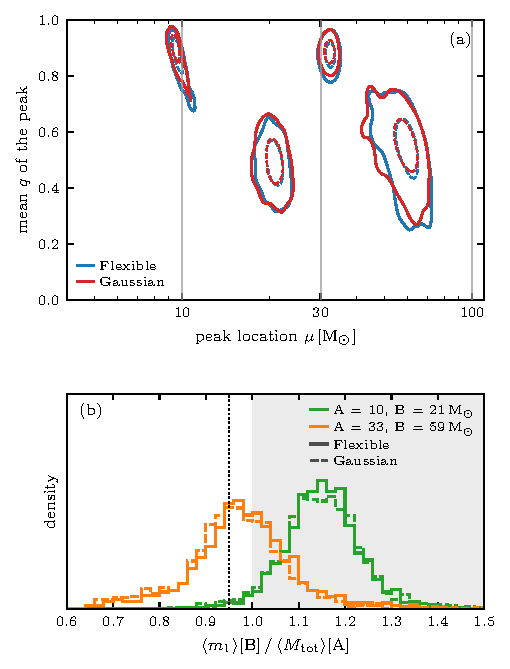
\includegraphics[width=\linewidth]{draft/plots/peak_bookkeeping.pdf}
    \caption{\todo{check how modes work} \todo{compare remnant distribution from 10Ms to 20M primaries. }\red{Draft caption. (a) Each peak's location $\mu$ against the mean mass ratio of the peak, from Gaussian + power-law fits to $p(m_1, q)$ in a window around each peak with no $q$ range imposed, per posterior draw; 90\% (solid) and 50\% (dashed) regions (Gaussian KDE) for the flexible (blue) and Gaussian (red) spin models. Two families: near-equal mass at $\sim$\featTen and $\sim$\featThirtyFive $\Msun$, $q \approx 0.5$ at $\sim$\featTwenty and $\sim$\featSixty $\Msun$. (b) The retained fraction $\langle m_1 \rangle[{\rm B}] / \langle M_{\rm tot} \rangle[{\rm A}]$, per draw: the mean primary mass of peak B (the location $\mu$ of its fitted Gaussian) over the mean total mass $M_{\rm tot} = m_1(1+q)$ of peak A, averaged over binaries drawn from A's fitted Gaussians in $m_1$ and $q$; pairs (A, B) = (\featTen, \featTwenty)\,\Msun and (\featThirtyFive, \featSixty)\,\Msun. Dotted: 0.95 ($\sim$5\% radiated); shaded: $> 1$. $\featTen \to \featTwenty$: $\pairTenTwentyRetainedMeanFlex$; $\featThirtyFive \to \featSixty$: $\pairThirtyFiveSixtyRetainedMeanFlex$. (\texttt{plots/peak\_bookkeeping.pdf}, one column, $\approx$130 words.)}}
    \label{fig: bookkeeping}
\end{figure}

\todo{the hierarchical-merger picture: each $q \sim 0.5$ feature is the second-generation partner of a near-equal-mass feature, in mass ratio, masses and spins. Summarize as a 2$\times$2: $\featTen \to \featTwenty$ (retained fraction $\pairTenTwentyRetainedModeFlex$, mild tension) and $\featThirtyFive \to \featSixty$ ($\pairThirtyFiveSixtyRetainedModeFlex$, consistent with $\sim$5\% radiated); in both pairs $\langle q \rangle$ drops from $\sim 0.85$ to $\sim 0.55$ and the $\chieff$ width grows. Why would the second generation pair with first-generation black holes of the same peak? Cite cluster predictions~\cite{Rodriguez:2019huv, Doctor:2019ruh, Kimball:2020opk, Gerosa:2021mno}. Implied 2G fraction at each mass?}

\heading{Discussion.}
The $\sim10\Msun$ peak does show a statistically significant preference for $\chieff > 0$, however, and the $\sim$ \featTwenty $\Msun$ peak is slightly more massive than the typical remnants from $\sim$ \featTen $\Msun$ peak \ac{BBH}. This suggests that not \textit{all} $\sim$ \featTen $\Msun$ \ac{BBH} are assembled dynamically, or that \jh{more complex dynamical theories are required, like that "not all dynamical bhs have isotropic spins paper from Davide's group", or dynamical environments evolve over cosmic time, perhaps 2G mergers today had higher z progenitors which had higher masses, e.g., \featTen $\Msun$ peak drifts a bit over cosmic time... something something metallicity and winds} the dynamical environments responsible for the $\sim$ \featTwenty $\Msun$ peak are at a different evolutionary period from the $\sim$ \featTen $\Msun$ dynamical mergers. 

\red{Target $\sim$350 words.
\begin{itemize}
\item Tentative, stated plainly. Posterior-only significance measures do not work in a model this flexible (random prior fields give fitted peaks 70--85\% of the time; SM).
\item A calibrated $p$-value needs mock catalogues (planned).
\item Forecast: $\sim$2--4$\times$ more events (the full O4 sample) for a decisive test.
\item Next: correlate redshift; channel-mixture interpretation (companion paper).
\item Excess over a local power law (SM): each peak stands above the chord in $(\ln m_1, \ln p)$ across its window in its own $q$ range, $P_{\rm loc} = \peakTenExcessPLocFlex\%$, $\peakTwentyExcessPLocFlex\%$, $\peakThirtyFiveExcessPLocFlex\%$, $\peakSixtyExcessPLocFlex\%$ (\featTen, \featTwenty, \featThirtyFive, \featSixty $\Msun$), and not in the other $q$ range ($P_{\rm loc} \approx 0.3$--0.6, SM Fig.): the off-diagonal $q$ slices are a built-in control for noise-fitting. Posterior probabilities, not $p$-values; the windows were chosen after seeing the field.
\end{itemize}}


\begin{acknowledgments}
\jh{acknowledgments}
\end{acknowledgments}

% PRL End Matter: check the current APS guidance on its placement (after the acknowledgments) and length.
\section*{End Matter}

The effective spin distribution has been found to correlate with several binary parameters: it broadens toward unequal masses~\cite{Callister:2021fpo, Adamcewicz:2022hce, Heinzel:2023hlb, LIGOScientific:2026ctl}, it broadens with redshift~\cite{Biscoveanu:2022qac, Heinzel:2023hlb}, and its width alternates narrow--broad--narrow--broad across the primary mass spectrum~\cite{Plunkett:2026pxt, Antonini:2025ilj, Tong:2025xir, Alvarez-Lopez:2026ymo}. Each of these correlations is usually measured with the spins conditioned on one binary parameter, with the rest of the population held fixed, and without assuming the mass, mass ratio or redshift are correlated. 


\textit{Mass ratio.} Averaged over primary mass, the width of the $\chieff$ distribution is $\sigma_{\chieff} = \chiQBroadSdQLoCoreFlex$ ($\chiQBroadSdQLoCoreGauss$) at $q = 0.35$, against $\chiQBroadSdQHiCoreFlex$ ($\chiQBroadSdQHiCoreGauss$) at $q = 0.85$, narrower near equal masses with probability $\chiQBroadProbCoreFlex\%$ ($\chiQBroadProbCoreGauss\%$), against $\chiQBroadProbPriorCoreFlex\%$ under the prior. This agrees with the linear and spline $\chieff \mid q$ models of \citet{LIGOScientific:2026ctl} (Fig.~\ref{fig: chi_eff width q}), and our models find it without assuming a functional form in $q$. In our population, the broadening comes from the two families of features: the narrow spin distributions of the \featTen and \featThirtyFive $\Msun$ features at $q \sim 1$ and the broad ones of the \featTwenty and \featSixty $\Msun$ features at $q \sim 0.5$, as argued explicitly in \citet{Vijaykumar:2026zjy}.

\textit{Primary mass.} The binary masses \textit{are} themselves correlated: the mass ratio distribution varies with primary mass, from $q \sim 1$ at the \featTen and \featThirtyFive $\Msun$ features to $q \sim 0.5$ at the \featTwenty and \featSixty $\Msun$ features (Fig.~\ref{fig: mass peaks}). We show below that a $\chieff$ width that depends explicitly only on mass ratio explains both the mass ratio and the primary mass correlations: the latter follows from the oscillating mass ratio. The converse also describes the data well: a width that oscillates \textit{explicitly} between narrow at $m_1\sim$ \featTen $\Msun$, broad at $m_1\sim$ \featTwenty $\Msun$, narrow at $m_1\sim$ \featThirtyFive $\Msun$, and broad at $m_1\sim$ \featSixty $\Msun$ without depending on mass ratio can produce the broadening with mass ratio as the \featTen and \featThirtyFive $\Msun$ features are at mass ratios close to $q\sim1$, and the \featTwenty and \featSixty $\Msun$ features are at $q\sim 0.5$. 
The data struggle to distinguish between these two cases \jh{include likelihoods for each}, however a model which allows both simultaneously prefers the mass ratio dependence over a primary mass dependence. This preference comes mostly from the \textit{Occam's factor}: a monotonic trend with mass ratio is simpler (larger prior volume) than an oscillatory trend with primary mass that just happens to align where the \featTen, \featTwenty, \featThirtyFive and \featSixty $\Msun$ features appear \jh{confirm with the $m_1$-only and $q$-only runs}. 

To compare the two, we fit a version of the \gaussianspins model in which each parameter of the spin distribution is additive in $\ln m_1$, $q$ and $z$,
\begin{equation}
    \theta(m_1, q, z) = \theta_0 + F_{\ln m_1}(\ln m_1) + F_q(q) + F_z(z),
    \label{eq: additive}
\end{equation}
for $\theta \in \{\mu_{\chieff}, \mu_{\chip}, \ln\sigma_{\chieff}, \ln\sigma_{\chip}, \tanh^{-1}\rho\}$, where $F_{\ln m_1}$, $F_q$ and $F_z$ are independent one-dimensional Mat\'ern fields. The model therefore can \textit{decide} if the data are best described by a population where the width evolves explicitly dependent on the primary mass, mass ratio, and/or the redshift. As described above, a broadening towards unequal mass ratios is degenerate with a narrow-broad-narrow-broad structure, aligned with the \featTen, \featTwenty, \featThirtyFive, and \featSixty $\Msun$ features. We will show both descriptions are more or less consistent, \jh{how does the $F_z$ only do?}

Figure~\ref{fig: additive} compares the explicit dependence (top) with the marginal one (bottom). The model places the explicit dependence on mass ratio: at fixed $m_1$ and $z$, the width is larger by a factor $\sim 3$ at $q \lesssim 0.6$ than at $q \approx 1$, and the marginal $\sigma_{\chieff}(q)$ has the same shape, falling from $\sim 0.25$ to $\sim 0.08$. The explicit dependence on primary mass is consistent with none: its median factor stays between $\sim 0.9$ and $1.4$ from 5 to $150\,\Msun$, with no narrow--broad--narrow--broad structure. It is also poorly constrained ($\times 0.5$--$4$ at 90\% near $20\,\Msun$), as expected if the data alone cannot distinguish the two descriptions. Yet the marginal $\sigma_{\chieff}(m_1)$ of the same model recovers that structure in full: it is $\sim 0.08$ at $\sim$ \featTen $\Msun$, $\sim 0.25$ at $\sim 18$--$20\,\Msun$, $\sim 0.12$ at $\sim$ \featThirtyFive $\Msun$ and $\sim 0.25$ above $\sim 50\,\Msun$. Since the mean $\chieff$ barely depends on $q$, the marginal width follows the mass ratio distribution: it is narrow where the binaries are near equal mass (the \featTen and \featThirtyFive $\Msun$ features) and broad where they are not (the \featTwenty and \featSixty $\Msun$ features). The non-additive models show the same: in both the \flexiblespins and \gaussianspins models, the width within a fixed band of mass ratio changes slowly with primary mass, and the oscillation appears only when the bands are combined (Fig.~\ref{fig: chi_eff width}). \red{Models with only one of the two dependences fit comparably well and reproduce much of the same marginal structure (SM), so the data do not cleanly separate a dependence on mass ratio from one on primary mass; they differ mainly in how sharply $\sigma_{\chieff}(q)$ falls near $q \approx 0.7$.}

The explicit mass ratio dependence is also the simpler physical picture. In the hierarchical-merger interpretation above, second-generation mergers are unequal mass and have broad, nearly symmetric $\chieff$ distributions~\cite{Vijaykumar:2026zjy}, whatever their mass, so a single cause produces both the broadening with mass ratio and the structure in $\sigma_{\chieff}(m_1)$. An explicit primary mass dependence would instead require the spins to change with mass in step with the mass ratio features. We do not expect the mass ratio itself to set the spins: both are set by how the binaries formed, and the mass ratio traces this better than the primary mass does. \red{In this picture neither $F_q$ nor $F_{\ln m_1}$ is the underlying description. If the population is a mixture of subpopulations, such as first- and second-generation mergers, with different distributions of primary mass, mass ratio and spin, then the width at each $(m_1, q)$ is set by the local fraction of each subpopulation. That fraction depends on both $m_1$ and $q$ and need not be separable, and because the subpopulations sit at different primary masses and mass ratios, either variable alone tracks it well. This is why the $F_q$-only and $F_{\ln m_1}$-only models fit comparably well, and why the joint model lies between them (SM). The two single-variable descriptions differ only where the subpopulations overlap: near-equal-mass binaries at $\sim \featTwenty$ or $\gtrsim 50\,\Msun$, and unequal-mass binaries at the \featTen\ and \featThirtyFive $\Msun$ features, where few events are observed so far.} The mean $\chieff$ shows one exception to the absence of an explicit primary mass dependence: a small excess of $\sim +0.02$ at $\sim 11\,\Msun$, which corresponds to the preference for $\chieff > 0$ at the \featTen $\Msun$ feature.

The additive model cannot represent interactions, for example a primary mass dependence only at unequal masses, so it does not rule them out. The non-additive models, which can, find little: the one exception is the width at $q \approx 1$, which rises above $\sim 50\,\Msun$ in all of our models (Fig.~\ref{fig: chi_eff width}). This may be a genuine dependence on primary mass, or a contribution from near-equal-mass mergers of two second-generation black holes. The precessing spin carries little information here: the explicit and marginal moments of $\chip$ are consistent with constant in $m_1$ and $q$ in all three redshift models. The exception is a rise of the mean $\chip$ from $\sim 0.2$ to $\sim 0.35$ below $z \approx 0.4$, which we do not interpret further.

\begin{figure}
    \centering
    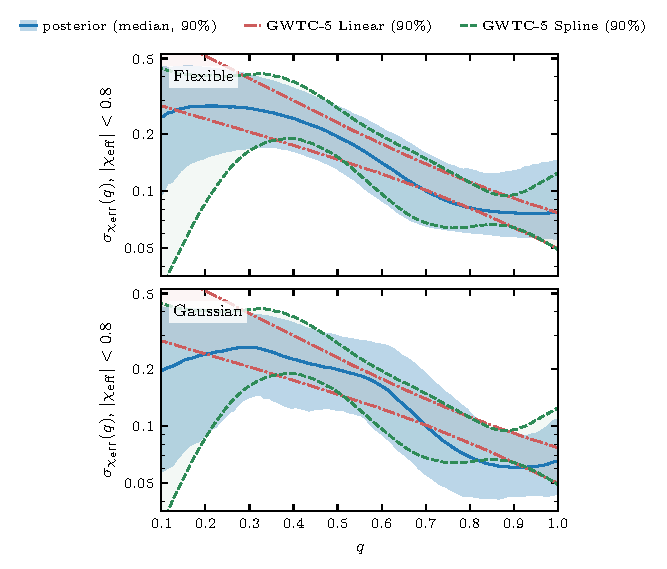
\includegraphics[width=\linewidth]{draft/plots/chi_eff_sd_q_core_lvk.pdf}
    \caption{\jh{we need to widen the actual figure so it fits the width of the legend, and we aren't wasting space}
    \red{Draft caption. The core width of the effective-spin distribution as a function of mass ratio, $\sigma_{\chieff}(q)$: the standard deviation of $p(\chieff \mid q, |\chieff| < 0.8)$, with the conditional averaged over $p(m_1 \mid q)$, for the \flexiblespins (top) and \gaussianspins (bottom) spin models (blue: posterior median and 90\% band). Lines: the 90\% intervals of the Gaussian width $\sigma_{\chieff}(q)$ in the GWTC-5 linear (red, dash-dotted) and spline (green, dashed) $\chieff \mid q$ models, over a faint fill. All four agree: the width falls from $\sim$0.2--0.3 at $q \lesssim 0.4$ to $\sim$0.08 near $q = 1$. The GWTC-5 widths are not restricted to $|\chieff| < 0.8$, so the comparison is approximate where the tails matter. Our models find this without a parametric form in $q$; the mean $\mu_{\chieff}(q)$ is flat and consistent with GWTC-5 (SM, \texttt{chi\_eff\_mean\_sd\_q\_core\_lvk.pdf}); the version with the spin prior is \texttt{chi\_eff\_sd\_q\_core\_prior.pdf}. (\texttt{plots/chi\_eff\_sd\_q\_core\_lvk.pdf}, one column.)}}
    \label{fig: chi_eff width q}
\end{figure}

\begin{figure}
    \centering
    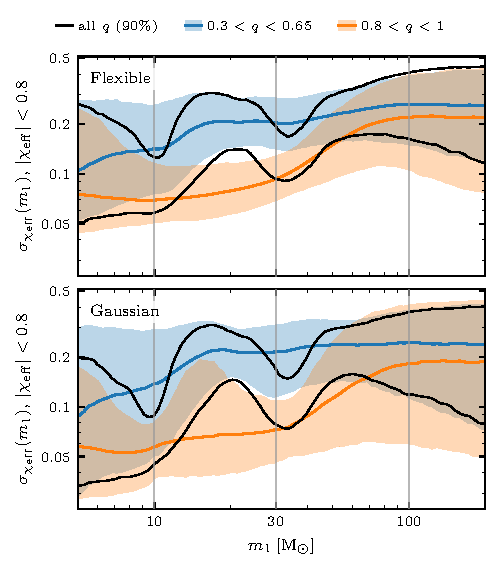
\includegraphics[width=\linewidth]{draft/plots/chi_eff_sd_m1_core.pdf}
    \caption{\red{Draft caption. The width of the effective-spin distribution at each primary mass, $\sigma_{\chieff}(m_1)$: the standard deviation of $p(\chieff \mid m_1, |\chieff| < 0.8)$, i.e.\ restricted to the core $|\chieff| < 0.8$ so that the poorly constrained tails do not set the width. Shown over all mass ratios (black lines: 90\% interval) and for $0.3 < q < 0.65$ (blue) and $0.8 < q < 1$ (orange) (90\% bands and medians), for the \flexiblespins (top) and \gaussianspins (bottom) spin models. The width is small at the near-equal-mass peaks ($\sim$\featTen and $\sim$\featThirtyFive $\Msun$) and large at $\sim$18--20 and $\gtrsim 45\,\Msun$, driven by the low-$q$ systems. The mean, $\mu_{\chieff}(m_1)$, is in the SM (\texttt{chi\_eff\_mean\_m1\_core.pdf}). (\texttt{plots/chi\_eff\_sd\_m1\_core.pdf}, one column.)}}
    \label{fig: chi_eff width}
\end{figure}

\begin{figure*}
    \centering
    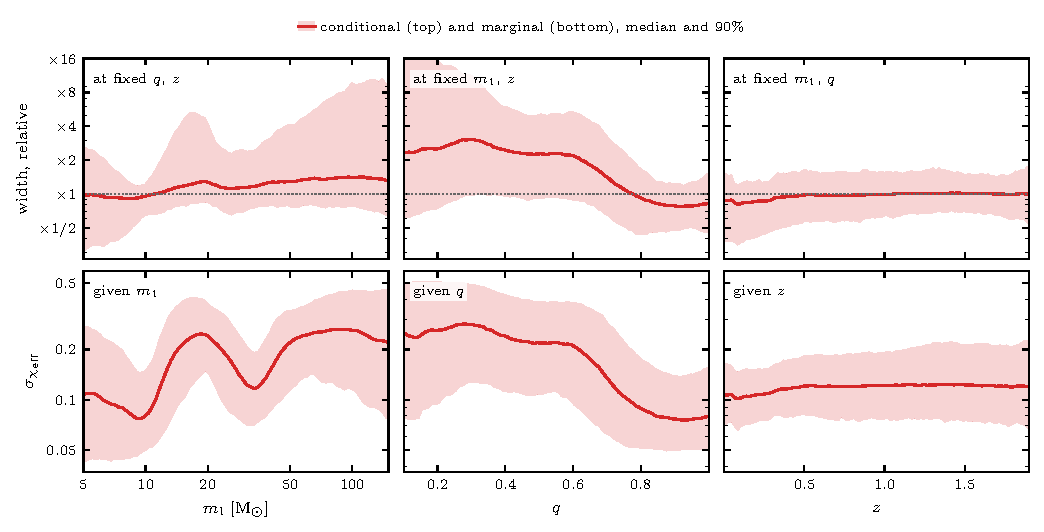
\includegraphics[width=\linewidth]{draft/plots/chi_eff_sd_conditional_marginal_additive.pdf}
    \caption{\red{Draft caption. The width of the $\chieff$ distribution in the additive \gaussianspins model, Eq.~\eqref{eq: additive}. Top: the conditional dependence on each of $m_1$, $q$ and $z$ at fixed values of the other two, $\exp[F - \langle F \rangle]$ for $\ln \sigma_{\chieff}$, relative to the population average (the overall scale is not identified). Bottom: the population marginals $\sigma_{\chieff}$ given $m_1$, $q$ and $z$ alone. Median and 90\%. The mass ratio dependence alone reproduces the narrow--broad--narrow--broad marginal $\sigma_{\chieff}(m_1)$; the conditional dependence on $m_1$ and $z$ is consistent with none.}}
    \label{fig: additive}
\end{figure*}

\bibliography{draft/main}

\end{document}
